\section{Correlation Estimation}

\begin{enumerate}[label=\alph*), leftmargin=*]
%% a)
\item
%

Figure \ref{fig:2_1_a} shows the biased (red) and unbiased (blue) estimates of the autocorrelation function (ACF) as well as the correlogram spectral estimates obtained for:
white gaussian noise (WGN), a noisy sinusoidal signal ($\sigma^{2} = 1$) and filtered white gaussian noise.

\begin{figure}[h]
    \centering
    \begin{subfigure}{0.49\textwidth}
        \centering
        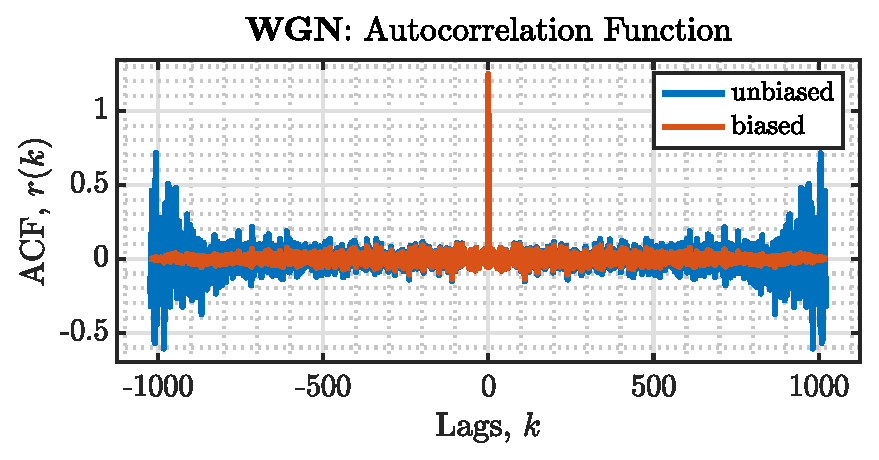
\includegraphics[height=1.5in]{report/parametric-and-line-spectra/correlation-estimation/assets/a/acf-WGN}
    \end{subfigure}
    ~
    \begin{subfigure}{0.49\textwidth}
        \centering
        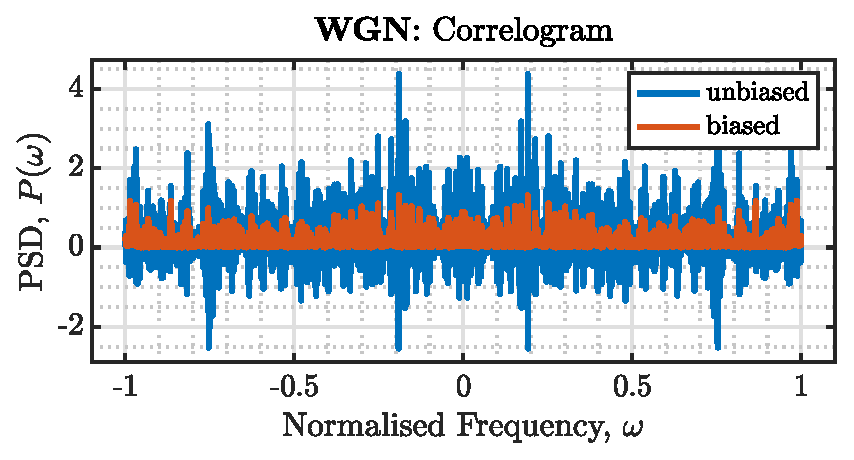
\includegraphics[height=1.5in]{report/parametric-and-line-spectra/correlation-estimation/assets/a/psd-WGN}
    \end{subfigure}
    ~
    ~
    \begin{subfigure}{0.49\textwidth}
        \centering
        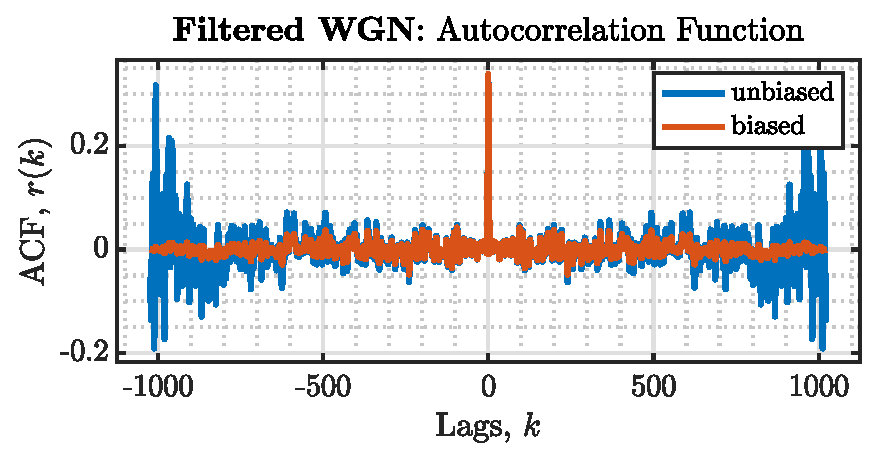
\includegraphics[height=1.5in]{report/parametric-and-line-spectra/correlation-estimation/assets/a/acf-Filtered_WGN}
    \end{subfigure}
    ~ 
    \begin{subfigure}{0.49\textwidth}
        \centering
        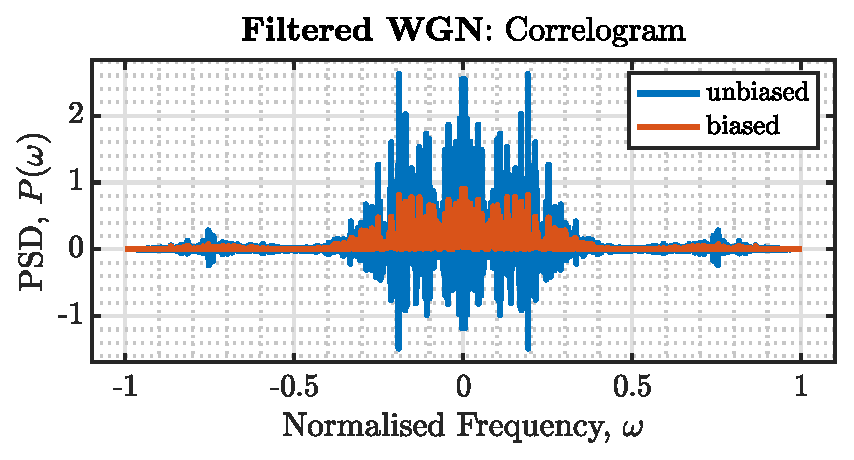
\includegraphics[height=1.5in]{report/parametric-and-line-spectra/correlation-estimation/assets/a/psd-Filtered_WGN}
    \end{subfigure}
    ~
    ~
    \begin{subfigure}{0.49\textwidth}
        \centering
        \includegraphics[height=1.5in]{report/parametric-and-line-spectra/correlation-estimation/assets/a/acf-Noisy_Sinewave}
    \end{subfigure}
    ~
    \begin{subfigure}{0.49\textwidth}
        \centering
        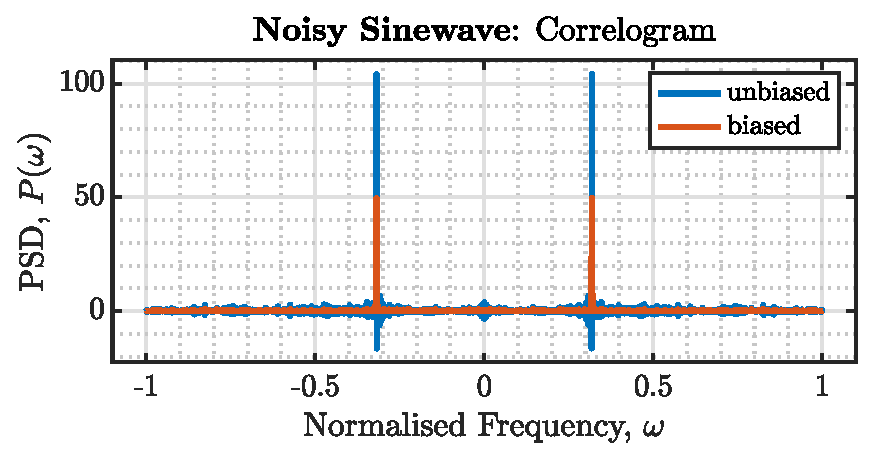
\includegraphics[height=1.5in]{report/parametric-and-line-spectra/correlation-estimation/assets/a/psd-Noisy_Sinewave}
    \end{subfigure}
    \caption{ACF and Correlogram: biased and unbiased estimates of various signals.}
    \label{fig:2_1_a}
\end{figure}

Regarding the ACF estimates, we verify that for small lags, $k \lessapprox 150$, the two estimates are very similar, but for larger lags 
the unbiased estimates increase in value while the biased estimates fade out to zero. We now show that the biased and unbiased ACF
estimates are obtained by windowing the ideal ACF $r_{xx}(k)$ with the Bartlett window, $w_{B}(k)$, and the rectangular window, $w_{R}(k)$, respectively.

\begin{align}
    \E[ \hat{r}_{biased}(k) ] &= \sum_{n=k+1}^{N} \frac{N - k}{N} r_{xx}(k) = w_{B}(k) r_{xx}(k) \\
    \E[ \hat{r}_{unbiased}(k) ] &= \sum_{n=k+1}^{N} \frac{N - k}{N - K} r_{xx}(k) = w_{R}(k) r_{xx}(k)
\end{align}

Thus, using the Fourier transform pair ACF-PSD, we obtain the expected values of the correlograms $\E[\hat{P}_{biased}]$ and $\E[\hat{P}_{unbiased}]$ as the convolution of
of the true power spectrum with the Fourier transform of the Bartlett and rectangular window, respectively. The Fourier transform of the rectangular window
is the $sinc$ function, which introduces \textbf{negative} values, and does not preserve the positive semi-definiteness of the PSD. On the other hand, the
Fourier transform of the Bartlett window is strictly non-negative\footnote{see figure \ref{fig:1_3_a_2} from Assignment 1}, guaranteeing positive semi-definiteness.
The correlograms in figure \ref{fig:2_1_a} verify our theoretical argument, where the unbiased estimates lead to negative PSD values while this is not the case for
the biased estimates.

%% b)
\item
%

Figure \ref{fig:2_1_b} illustrates the periodogram of 100 realisations of the random process $x(n)$,
as well as the ensemble mean and standard deviation, where:

\begin{equation}
    x(n) = 1.5 sin(2 \pi 0.3 n) + sin(2 \pi 0.6 n) + 2 sin(2 \pi 0.9 n) + w(n) \quad w \sim \mathcal{N}(0, 1)
\end{equation}

\begin{figure}[h]
    \centering
    \begin{subfigure}{0.49\textwidth}
        \centering
        \includegraphics[height=1.5in]{report/parametric-and-line-spectra/correlation-estimation/assets/b/psd_mean}
    \end{subfigure}
    ~
    \begin{subfigure}{0.49\textwidth}
        \centering
        \includegraphics[height=1.5in]{report/parametric-and-line-spectra/correlation-estimation/assets/b/psd_std}
    \end{subfigure}
    \caption{Correlogram: mean and standard deviation of $x(n)$.}
    \label{fig:2_1_b}
\end{figure}

When the biased ACF estimate is used, the obtained correlogram is an \textbf{inconsistent estimator} since:

\begin{equation}
    \Var[\hat{P}_{biased}(f)] = P_{xx}^{2}(f) \bigg[ 1 + \bigg(\frac{sin(2 \pi N f)}{N sin(2 \pi f)}\bigg)^{2} \bigg]
\end{equation}

and as a result when $N \rightarrow \infty$, $\Var[\hat{P}_{biased}(f)] \rightarrow P_{xx}^{2}(f) \gg 0$. This also explains the increased standard deviation of the periodogram
at the peak frequencies of the ideal PSD, $P_{xx}(f)$, of the process.

%% c)
\item
%

The experiments are repeated and the periodograms are expressed in $dB$ this time, as illustrated in figure \ref{fig:2_1_c}.
Interestingly, the variance close to the peak frequencies, $f = 0.3,\ 0.6,\ 0.9\ Hz$, is decreased.
This is a counter-intuitive result, but it can be explained by the logarithmic function's gradient ($\frac{1}{x}$).
Fluctuations around zero are significantly amplified, while values greater than $1$ are attenuated (sub-linear trend). Consequently, since the power at peak frequencies is much greater
than $1$, its variance is squeezed, while at all other frequencies power is concentrated around zero, leading to amplified variance.

Clearly, this is an advantageous representation, since at frequencies of interest the spread-out is reduced and the interpretation of the periodograms is easier.

\begin{figure}[h]
    \centering
    \begin{subfigure}{0.49\textwidth}
        \centering
        \includegraphics[height=1.5in]{report/parametric-and-line-spectra/correlation-estimation/assets/c/psd_mean}
    \end{subfigure}
    ~
    \begin{subfigure}{0.49\textwidth}
        \centering
        \includegraphics[height=1.5in]{report/parametric-and-line-spectra/correlation-estimation/assets/c/psd_std}
    \end{subfigure}
    \caption{Correlogram: mean and standard deviation of $x(n)$ in $dB$.}
    \label{fig:2_1_c}
\end{figure}

%% d)
\item
%

Figure \ref{fig:2_1_d} shows the periodograms of complex exponential signals (two sine waves) in noise for different number of samples and therefore frequency resolutions.
As expected, for small number of samples ($n \leq 40$) the two peaks cannot be distinguished but for larger values ($n \geq 45$) the two peaks are visible.
This observation agrees with theory, since the resolution of the (standard) periodogram is given by $\Delta f = \frac{0.89}{N}$ and the two complex signals have
frequencies $f_{1} = 0.3\ Hz$ and $f_{2} = 0.32\ Hz$, hence discrimination is possible when:

\begin{equation}
    \Delta f \leq f_{2} - f_{1} \Longrightarrow N \geq \frac{0.89}{f_{2} - f_{1}} = \frac{0.89}{0.32 - 0.3} = 44.5
\end{equation}

\begin{figure}[h]
    \centering
    \begin{subfigure}{0.49\textwidth}
        \centering
        \includegraphics[height=1.5in]{report/parametric-and-line-spectra/correlation-estimation/assets/d/complex_exponentials-1}
    \end{subfigure}
    ~
    \begin{subfigure}{0.49\textwidth}
        \centering
        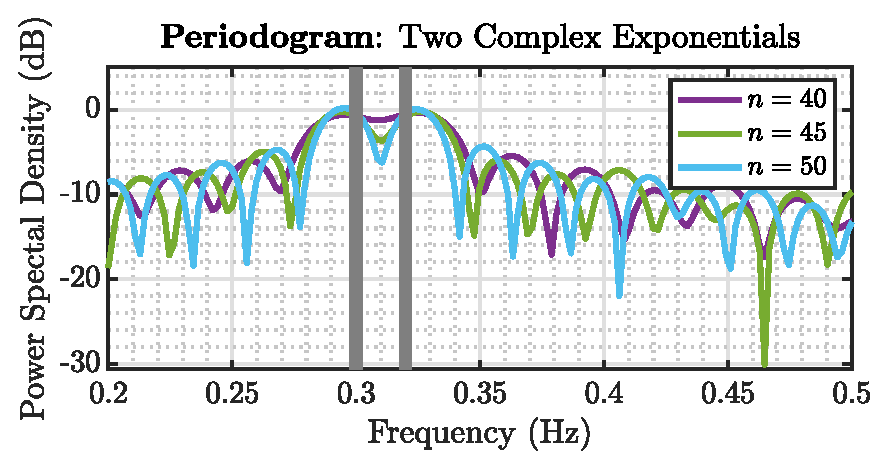
\includegraphics[height=1.5in]{report/parametric-and-line-spectra/correlation-estimation/assets/d/complex_exponentials-2}
    \end{subfigure}
    \caption{Periodogram: frequency resolution and peak identification.}
    \label{fig:2_1_d}
\end{figure}

Hence, despite the simplicity of the signals under investigation (two sine waves), the periodogram fails to adequately estimate their power spectral density when a small number
of samples is available. Therefore, alternative methods (i.e subspace methods) must be used in these cases.

%% e)
\item
%

The MUltiple SIgnal Classification algorithm (MUSIC) estimates the spectral density of a signal, using a \textbf{subspace} method. It assumes that the signal, $x(n)$,
consists of $p$ complex exponentials in the presence of Gaussian white noise. Given an autocorrelation matrix, $\mathbf{R}_{xx} \in \sR^{M \times M}$,
if its eigenvalues are sorted in decreasing order, the eigenvectors corresponding to the $p$ largest eigenvalues (i.e. directions of largest variability) span the signal subspace, $\mathbf{R}_{s}$.
The remaining $M-p$ eigenvectors span the orthogonal space, $\mathbf{R}_{n}$, where there is only noise.
Let the noise eigenvectors $\vv_{i}$ and the helper vector $\ve$ such that:

\begin{equation}
    \vv_{i}, \quad i = p+1, \ldots, M \qquad \text{and} \qquad
    \ve = 
    \begin{bmatrix}
        1 & e^{jw} & e^{j2w} & \cdots &  e^{j(M-1)w}
    \end{bmatrix}^{T}
\end{equation}

then the MUSIC spectral estimate $\hat{P}_{MU}$ is given by:

\begin{equation}
    \hat{P}_{MU}(e^{jw}) = \frac{1}{\sum_{i=p+1}^{M} |\ve^{H} \vv_{i}|^{2}}
\end{equation}

where at signal frequencies $w_{1},\ \ldots,\ w_{k},\ \ldots,\ w_{p}$ the noise eigenvectors $\vv_{i}$ and the signal eigenvectors $\ve_{k}$ will be orthogonal (since $\mathbf{R}_{xx}$ is Hermitian)
and therefore $\hat{P}_{MU}$ will have $p$ peaks, as expected for a spectrum estimator of $p$ complex exponentials.

The modified autocorrelation matrix $\mathbf{R}_{xx}$ with $M = 14$ is obtained using MATLAB command:

\begin{equation*}
    \mathtt{[X,Rxx] = corrmtx(x, 14, "mod")}
\end{equation*}

which is used by the MUSIC algorithm for spectral estimation

\begin{equation*}
    \mathtt{[S,F] = pmusic(Rxx, p, [ ], 1, "corr")}
\end{equation*}

where \texttt{p} is the signal subspace dimensionality, a hyperparameter that must be tuned/selected.

In figure \ref{fig:2_1_e}, the 100 realisations overlay of a two complex exponentials signal ($f_{1} = 0.3\ Hz$ and $f_{2} = 0.32\ Hz$) MUSIC spectrum estimate is provided,
alogn with their standard deviation, for different values of hyperparameter $p$.

\begin{figure}[h]
    \centering
    \centering
    \begin{subfigure}{0.49\textwidth}
        \centering
        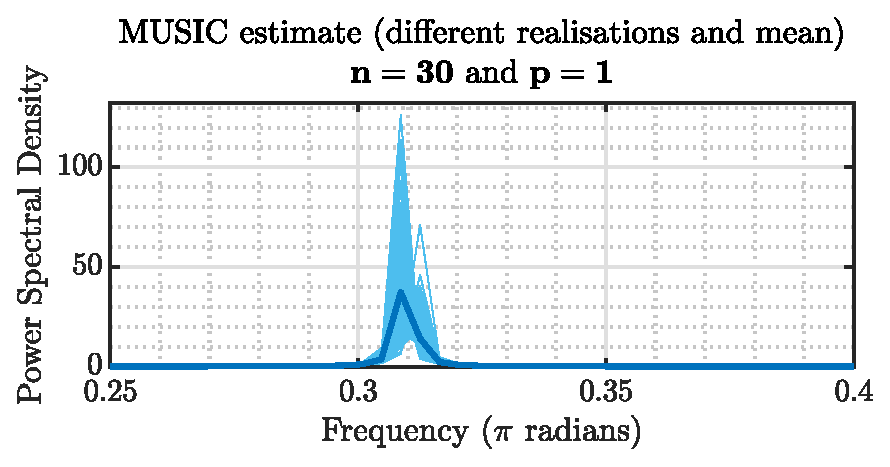
\includegraphics[height=1.5in]{report/parametric-and-line-spectra/correlation-estimation/assets/e/MUSIC_mean-p_1}
    \end{subfigure}
    ~
    \begin{subfigure}{0.49\textwidth}
        \centering
        \includegraphics[height=1.5in]{report/parametric-and-line-spectra/correlation-estimation/assets/e/MUSIC_std-p_1}
    \end{subfigure}
    ~
    ~
    \begin{subfigure}{0.49\textwidth}
        \centering
        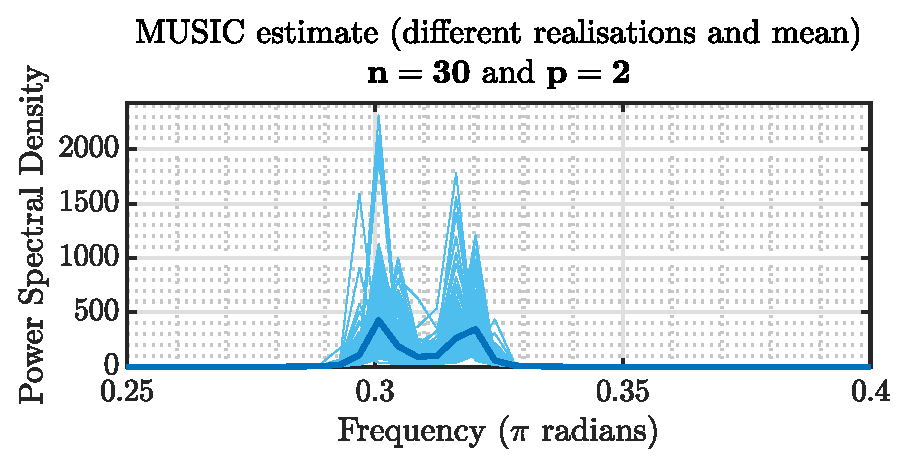
\includegraphics[height=1.5in]{report/parametric-and-line-spectra/correlation-estimation/assets/e/MUSIC_mean-p_2}
    \end{subfigure}
    ~ 
    \begin{subfigure}{0.49\textwidth}
        \centering
        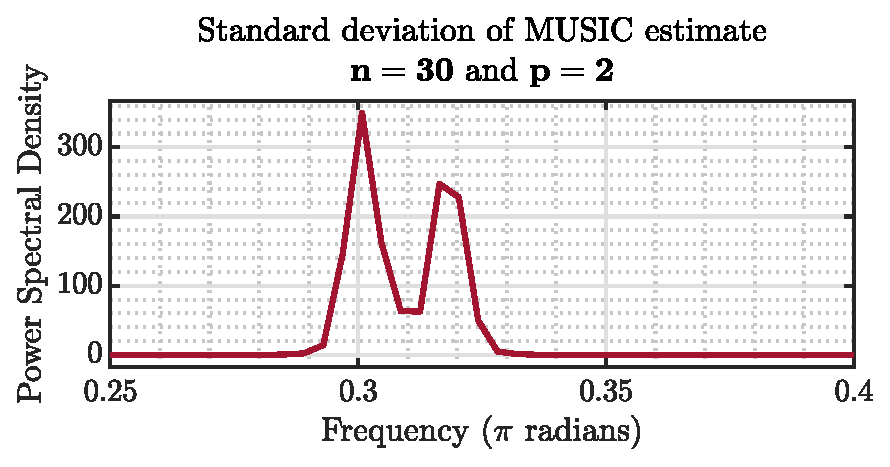
\includegraphics[height=1.5in]{report/parametric-and-line-spectra/correlation-estimation/assets/e/MUSIC_std-p_2}
    \end{subfigure}
    ~
    ~
    \begin{subfigure}{0.49\textwidth}
        \centering
        \includegraphics[height=1.5in]{report/parametric-and-line-spectra/correlation-estimation/assets/e/MUSIC_mean-p_3}
    \end{subfigure}
    ~
    \begin{subfigure}{0.49\textwidth}
        \centering
        \includegraphics[height=1.5in]{report/parametric-and-line-spectra/correlation-estimation/assets/e/MUSIC_std-p_3}
    \end{subfigure}
    \caption{MUSIC: spectral estimation of two complex exponentials and signal space size $p$.}
    \label{fig:2_1_e}
\end{figure}

Despite the small number of samples available ($n = 30$) and thus the poor frequency resolution, the algorithm successfully identifies the two
frequency components at $f_{1}$ and $f_{2}$, when $p=2$ is selected, unlike the periodogram that requires a larger amount of samples.
Similar to the periodogram, the standard deviation of the estimator increases closer to the peak values, but most importantly, the reliability
of the estimator deteriorates significantly when $p$ is not matched with the nature of signal $x(n)$.

To sum up, MUSIC method is very powerful when a small number of samples is available but its chief disadvantage is that it requires the number of components $p$ to be known in advance,
so \textbf{it cannot be used in more general cases}, when prior knowledge of the signal is not provided. On the other hand, the periodogram needs
a finer frequency resolution to detect closely-spaced sine waves (larger $n$), but it does not require any knowledge about the signal $x(n)$.

%
\end{enumerate}